\chapter{Icicle, a language for push queries}
\label{part:icicle}


\newcommand\mi[1]         {\mathit{#1}}

\newcommand\NN  {\mathtt{Int}}
\newcommand\BB  {\mathtt{Bool}}
\newcommand\lam[1]         {\lambda{}#1.~}

\newcommand\GrammarDefTab  {\> $::=$ \>}
\newcommand\GrammarAlt  {\\ \> $~~|$ \>}


\newcommand\If[3] {\tt{if}~#1~\tt{then}~#2~\tt{else}~#3}
\newcommand\Ifnbot[3] {\If{#1~\not=~\bot}{#2}{#3}}

\newcommand\sref[1] {~(\S\ref{#1})}

\newcommand\arrayZ[1]
{ \begin{array}{l}
  #1
  \end{array}
}

\newtheorem{lemma}{Lemma}

%!TEX root = ../Main.tex
\newcommand\SourceStepX[4]
{                   #1~|~#2~\vdash~#3~\Downarrow~~#4
}

\newcommand\SourceStepXP[3]
{ \SourceStepX{\mathtt{Pure}}{#1}{#2}{#3} }
\newcommand\SourceStepXE[3]
{ \SourceStepX{\mathtt{Element}}{#1}{#2}{#3} }
\newcommand\SourceStepXA[3]
{ \SourceStepX{\mathtt{Aggregate}}{#1}{#2}{#3} }

\newcommand\Tau T
\newcommand\TauMode M
\newcommand\TauFun F
\newcommand\RawMode N

% this was lowercase sigma, but lambda sigma doesn't look like a binding
\newcommand\store s

\newcommand\VValue[1]
{ \tt{Value}~#1 }
\newcommand\VStream[1]
{ \tt{Stream}~#1 }
\newcommand\VFold[3]
{ \tt{Fold}~#1~#2~#3 }

\newcommand\TypeWf[3]
{ #1~\vdash~#2~:_k~#3
}

\newcommand\Typecheck[3]
{                   #1
        ~\vdash~    #2~:~#3
}

\newcommand\TypecheckP[2]
{                   #1~:_P~#2
}

\newcommand\TypecheckApp[3]
{                   #1~\bullet~#2~:~#3
}

\newcommand\TypecheckS[3]
{                   #1
        ~\vdash~    #2
        ~\dashv~    #3
}





\newcommand\CoreComp[4]
{                   #1 ~\xRightarrow{Core}~ #2 ~|~ #3 ~|~ #4
}



% We present Icicle, a pure streaming query language which statically guarantees that multiple queries over the same input stream are fused. We use a modal type system to ensure that fused queries can be computed incrementalally, and a fold-based intermediate language to compile down to efficient C code. We present production benchmarks demonstrating significant speedup over existing queries written in R, and on par with the Unix tools \texttt{grep} and \texttt{wc}.

%!TEX root = ../Main.tex
\label{icicle:s:Introduction}

This chapter presents Icicle, a domain-specific language for writing queries as push streams.
This work was first published as \citet{robinson2016icicle}, and was performed in collaboration with a machine-learning company called Ambiata.
At Ambiata, we perform feature generation for machine-learning applications by executing many thousands of simple queries over terabytes worth of compressed data.\footnote{In 2018, this was a lot of data.}
For such applications, we must automatically fuse these separate queries and be sure that the result can be executed in a single pass over the input.
We also ingest tens of gigabytes of new data per day, and must incrementally update existing features without recomputing them all from scratch.
Our feature generation process is executed in parallel on hundreds of nodes on a cloud based system, and if we performed neither fusion nor incremental update then the cost of the computation would begin to exceed the salaries of the developers.

The contributions of this chapter are:
\begin{itemize}
\item
  We motivate the use of Icicle by extending the previous ``gold panning'' queries (\cref{icicle/gold-panning});

\item
  We present Icicle, a domain-specific language that guarantees any set of queries on a shared input table can be fused, and allows the query results to be updated as new data is received (\cref{icicle:s:IcicleSource});

\item
  We present a fold-based intermediate language, which allows the query fusion transformation to be a simple matter of appending two intermediate programs, and exposes opportunities for common subexpression elimination (\cref{icicle:s:IcicleCore});

\item
  We present benchmarks of Icicle compiled code running in production (\cref{icicle:s:Benchmarks}). 
\end{itemize}

\section{Gold panning with Icicle}
\label{icicle/gold-panning}

In the following example queries, we extend the daily stock price records from \cref{taxonomy/gold-panning} to contain the open price and the close price for the day.
As Icicle uses push streams, the queries we write have a single input stream of the prices for a particular company; Icicle cannot express the @priceOverMarket@ example, which contains multiple input streams.
Suppose we want to compute the number of days where the open price exceeded the close price, and vice versa.
We also want the mean of the open price for days in which the open price exceeded the close price.
In Icicle, we write the three queries as follows:

\begin{icicle}
table stocks { open : Int, close : Int }
query 
  more = filter open > close of count;
  less = filter open < close of count;
  mean = filter open > close of sum open / count;
\end{icicle}

In the above code, (@open > close@) and (@close < open@) are filter predicates, and @count@ counts how many times the predicate is true.
The input table, @stocks@, defines the open and close prices as @Int@s.
In Icicle, input tables have an implicit time field and the input stream is sorted chronologically.

We can express the same three queries using the push streams from \cref{taxonomy/push}, as in the following program:

\begin{haskell}
data Record = Record
 { time :: Time, open :: Int, close :: Int }

queries :: IO (Push Record (Int,Int,Int))
queries = do
  more_count <- count
  let more = filter (\r -> open r > close r) more_count

  less_count <- count
  let less = filter (\r -> open r < close r) less_count

  mean_sum   <- foldl (+) 0
  mean_count <- count
  let mean = filter (\r -> open r > close r)
                    (div <$> contramap open mean_sum <*> mean_count)
  return ((,,) <$> more <*> less <*> mean)
\end{haskell}

Despite the syntactic differences, the two programs have roughly the same structure in terms of the three queries.
The three instances of \Hs@count@ are constructed as monadic \Hs@IO@ operations, because each count uses a separate mutable reference.
The applicative functor syntax is used to divide the sum by the count in the @mean@ query, because the division is performed on the result of the push stream.
Icicle does not use the applicative syntax, as it uses a modal type system to infer which computations are performed on the result of the stream, as described in \cref{icicle:s:ElementsAndAggregates:TypeSystem}.

In this example, both @more@ and @mean@ compute the count with the same filter predicate.
When the same computation is used by multiple queries, we would like to compute the value only once and share the result among all the queries that use it.
Common subexpression elimination (CSE) removes some duplicate computations but, as its name suggests, it is limited to structural subexpressions~\cite{chitil1997uncommon}.
Neither of the filtered counts is a subexpression of the other, so common subexpression elimination will not remove the duplicate computation.
In Icicle, we remove this duplicate work by first converting queries to an intermediate language, described in \cref{icicle:s:IcicleCore}.
This intermediate language decomposes the query into individual folds, exposing the opportunities for common subexpression elimination.

If we were using an existing database implementation, we could convert all three queries to a single query in a back-end language like SQL, but doing so by hand is tedious and error prone.
As the three queries use different filter predicates, we cannot use a single @SELECT@ statement and a @WHERE@ expression to implement the filter.
We must instead lift each predicate to an expression-level conditional and compute the count by summing the conditional:

\begin{sql}
  SELECT SUM(IF(open > close, 1,    0))
       , SUM(IF(open < close, 1,    0))
       , SUM(IF(open > close, open, 0))
       / SUM(IF(open > close, 1,    0))
  FROM stocks;
\end{sql}

% As we see, the result of query fusion tends to have many common sub expressions, and we wish to guarantee that the duplicates in the fused result are eliminated.

Joint queries such as the stocks example can be evaluated in a streaming, incremental fashion, which allows the result to be updated as we receive new data.
As a counter-example, suppose we have a table with two fields @key@ and @value@, and we wish to find the mean of values whose key matches the last one in the table.
We might try something like:

\begin{icicle}
  table kvs { key : Date; value : Int }
  query avg = let k = last key
              in  filter (key == k) of mean value;
\end{icicle}

Unfortunately, although the \emph{result} we desire is computable, the \emph{algorithm} implied by the above query cannot be evaluated incrementally.
When we are streaming through the table we always have access to the last key in the stream, but finding the rows that match this key requires streaming the table again from the start.
We need a better solution.

% , and are on par with standard Unix utilities.
% that conceptually perform less work.
%\ben{I think this clause confuses the contribution. If if Icicle is "on par" with standard unix utilities, then why not just use those standard utilities? The point is that with Icicle we can also fuse multiple queries, and the fused code should be at least as good as the unix utils. However, fusing two instances of 'wc' won't be exactly 2x fast then running them sequentially, but still better than actually running them sequentially. There's no space to discuss the details in the intro.

Icicle is related to stream processing languages such as Lucy~\cite{mandel2010lucy} and Streamit~\cite{thies2002streamit}, except we forgo the need for clock and deadlock analysis.
Icicle is also related to work on continuous queries~\cite{arasu2003cql}, where query results are updated as rows are inserted into the source table, except we can also compute arbitrary reductions and do not need to handle deleted source rows.
We discuss these points in more detail in \cref{icicle:s:Conclusion}.
Our implementation is available at \url{https://github.com/amosr/icicle}.
As of 2018, this implementation is still running in production in the machine-learning pipeline at Ambiata.

%!TEX root = ../Main.tex

% ---------------------------------------------------------
\section{Elements and aggregates}
\label{icicle:s:ElementsAndAggregates}
To allow incremental computation, all Icicle queries must execute in a single pass over the input stream.
Sadly, not all queries \emph{can} be executed in a single pass: the key examples are queries that require random access indexing, or otherwise need to access data in an order different to what the stream provides.
However, as we saw in the previous section, although a particular \emph{algorithm} may be impossible to evaluate in a streaming fashion, the desired \emph{value} may well be computable, if only we had a different algorithm.
Here is the unstreamable example from the previous section again:
\begin{icicle}
  table kvs { key : Date; value : Int }
  query meanOfLatest
   = let k = last key in
     filter (key == k) of mean value;
\end{icicle}

The problem is that the value of \Ic@last key@ is only available once we have reached the end of the stream, but \Ic@filter@ needs this value to process the very first element in the same stream.
We distinguish between these two access patterns by giving them different names: we say that (@last key@) is an \emph{aggregate}, because to compute it we must have consumed the \emph{entire stream}, whereas the filter predicate is an \emph{element}-wise computation because it only needs access to the current element in the stream.

The trick to compute our average in a streaming fashion is to recognise that \Ic@filter@ selects a particular subset of values from the input, but the value computed from this subset depends only on the values in that subset, and no other information. Instead of computing the mean of a single subset whose identity is only known at the end of the stream, we can instead compute the mean of \emph{all possible subsets}, and return the required one once we know what that is:
\begin{icicle}
  table kvs { key : Date; value : Int } 
  query meanOfLatest
   = let k    = last  key in
     let avgs = group key of mean value in
     lookup k avgs
\end{icicle}

Here we use the \Ic@group@ construct to assign key-value pairs to groups as we obtain them, and compute the running mean of the values of each group. The \Ic@avgs@ value becomes a map of group keys to their running means. Once we reach the end of the stream we will have access to the last key and can lookup the final result.
%% Review #1:
%% In Section 3 I kept looking for a definition of the “last” function, which takes an important role in the Introduction.
%% In Section 4, I found the definition. It would help the reader to give a small note early in Section 2 or 3 that “last”, “mean”, “sum” are user-level (i.e. non-primitive) functions whose definition will be given in Section 4.
Evaluation and typing rules are defined in~\cref{icicle:s:IcicleSource}, while the user functions \Ic@last@ and \Ic@mean@ are defined in~\cref{icicle:s:IcicleCore}.


% ---------------------------------------------------------
\subsection{The stage restriction}
To ensure that Icicle queries can be evaluated in a single pass, we use a modal type system inspired by staged computation~\cite{davies2001modal}.
We use two modalities, \Ic@Element@ and \Ic@Aggregate@.
Values of type \Ic@Element@~$\tau$ are taken from the input stream on a per-element basis, whereas values of type \Ic@Aggregate@~$\tau$ are available only once the entire stream has been consumed.
In the expression (\Ic@filter (key == k) of mean value@), the variable \Ic@key@ has type \Ic@Element Date@ while \Ic@k@ has type \Ic@Aggregate Date@.
Attempting to compile the unstreamable query in Icicle will produce a type error complaining that elements cannot be compared with aggregates.

The types of pure values, such as constants, are automatically promoted to the required modality.
For example, if we have the expression (\Ic@open == 1@), and the type-checking environment asserts that the variable \Ic@open@ has type \Ic@Element Int@, then the constant @1@ is automatically promoted from type \Ic@Int@ to type \Ic@Element Int@.


% ---------------------------------------------------------
\subsection{Finite streams and synchronous data flow}
In contrast to synchronous data flow languages such as {\sc Lustre}~\cite{halbwachs1991synchronous}, the streams processed by Icicle are conceptually finite in length.
Icicle is fundamentally a query language, which queries finite tables of data held in a non-volatile store, but does so in a streaming manner.
{\sc Lustre} operates on conceptually infinite streams, such as those found in real-time control systems (like to fly aeroplanes).
In Icicle, the ``last'' element in a stream is the last one that appears in the table on disk.
In {\sc Lustre}, the ``last'' element in a stream is the one that was most recently received.
If the unstreamable query from \cref{icicle:s:ElementsAndAggregates} were converted to {\sc Lustre} syntax then it would execute, but the filter predicate would compare the last key with the most recent key from the stream, which is the key itself.
The filter predicate would always be true, and the query would return the mean of the entire stream.
Applying the Icicle type system to our queries imposes the natural stage restriction associated with finite streams, so there are distinct ``during'' (element) and ``after'' (aggregate) stages.


% ---------------------------------------------------------
\subsection{Incremental update}
Suppose we query a large table and record the result.
Tomorrow morning, we receive more data and add it to the table.
We would like to update the result without needing to process all data from the start of the table.
We can do this by remembering the values of all intermediate aggregates that were computed in the query, and updating them as new data arrives.
In the \Ic@meanOfLatest@ example from \cref{icicle:s:ElementsAndAggregates}, these aggregates are \Ic@k@ and \Ic@avgs@. 

We also provide impure contextual information to the query, such as the current date, by assigning it an aggregate type.
As element-wise computations cannot depend on aggregate computations, we ensure that reused parts of an incremental computation are the same regardless of which day they are executed.


% ---------------------------------------------------------
\subsection{Bounded buffer restriction}
\label{icicle:s:IcicleSource:bounded}
Icicle queries process tables of arbitrary size that may not fit in memory.
As with other streaming models, each query must execute without requiring buffer space proportional to the size of the input.
As a counterexample, here is a simple list function which cannot be executed in a streaming manner without reserving a buffer of the same size as the input:
\begin{haskell}
unbounded :: [Int] -> [(Int,Int)]
unbounded xs = zip (filter (> 0) xs) (filter (< 0) xs)
\end{haskell}

This function takes an input list \Ic@xs@, and pairs the elements that are greater than zero with those that are less than zero.
If we try to convert this computation to a single-pass streaming implementation, it requires an unbounded buffer: if the stream contains $n$ positive values followed by $n$ negative values, then all positive values must be buffered until we reach the negative ones, which allow output to be produced.

%% Review #1
%% It’s not clear what’s meant by “In Icicle, queries that would require unbounded buffering cannot be written”.
%% My understanding is that they can be written, but we would get a runtime error because the buffer would eventually become too big to fit the memory. Is this right?
% change to "statically outlawed by the type system": I think that's unambiguous.

In Icicle, queries that would require unbounded buffering are statically outlawed by the type system, with one major caveat that we will discuss in a moment.
Because Icicle is based on the push streams described in \cref{taxonomy/push}, the stream being processed (such as \Ic@xs@ above) is implicit in each query.
Constructs such as \Ic@filter@ and \Ic@fold@ do not take the name of the input stream as an argument, but instead operate on the stream defined in the context.
Icicle language constructs describe \emph{how elements from the stream should be aggregated}, but the order in which those elements are aggregated is implicit, rather than being definable by the body of the query.
In the expression (\Ic@filter p of mean value@), the term (\Ic@mean value@) is applied to stream values which satisfy the predicate \Ic@p@, but the values to consider are supplied by the context.

Finally, our major caveat is that the \Ic@group@ construct we used in \cref{icicle:s:ElementsAndAggregates} uses space proportional to the number of distinct \emph{keys} in the input stream.
For our applications, the keys are commonly company names, customer names, and days of the year.
Our production system knows that these types are bounded in size, and that maps from keys to values will fit easily in memory.
Attempting to group by values of a type with an unbounded number of members, such as a \Ic@Real@ or \Ic@String@, results in a compile-time warning.

% Grouping by types with an unbounded number of members, such as \Ic@Real@ or \Ic@String@ can be undesirable, and we wish to outlaw this in a future version of our production compiler.

% BEN: "Can be undesirable" is too imprecise. What will happen is that an entry will be added to the map for every key, and if there are more keys than will fit in memory then the query will run out of memory. Surely adding the mentioned warning to the compiler would not be difficult? If it's easy then saying it's done sounds much better than "we intend to". We need to have a solid story about this point. One of the key contributions of Icicle is that it does not require ``unbounded buffering'', but if you're grouping by arbitrary values from the input stream then it clearly does.


% ---------------------------------------------------------
\subsection{Source language}
\label{icicle:s:IcicleSource}

The grammar for Icicle is given in \cref{icicle:fig:source:grammar}.
Value types ($T$) include numbers, booleans and maps; some types such as \Ic@Real@ and \Ic@String@ are omitted.
Modal types ($\TauMode$) include the pure value types, and modalities associated with a value type.
%% Review 3:
%% In Section 3, the description of function types is confusing.
%% The authors state, "Function types F include non-function modal types, and functions from modal type to function type."
%% It appears from Figure 1 that function types do not include non-function modal types (syntactic category M), and include only functions from modal type(s) to *modal* type.
Function types ($\TauFun$) include functions with any number of modal type arguments to a modal return type.
As Icicle is a first-order language, function types are not value types.
%!TEX root = ../Main.tex

\begin{figure}

\begin{tabbing}
MMMM \= MM \= MMM \= MM \= MMMMMM \= \kill
$\mi{T}$
\GrammarDefTab
  $@Int@~|~@Bool@~|~@Map@~T~T~|~(T~\times~T)$
\\
$\mi{\TauMode}$
\GrammarDefTab
  $T~|~@Element@~T~|~@Aggregate@~T$
\\
$\mi{\TauFun}$
\GrammarDefTab
  $\ov{(\TauMode)}~\to~\TauMode$
\\
\\

$\mi{Table}$
\GrammarDefTab
  $@table@~x~@{@~\ov{(x~:~T;)}~@}@$
\\
\\

$\mi{Exp}$, $e$
\GrammarDefTab
  $x~|~V~|~\mi{Prim}~\ov{\mi{Exp}}~|~x~\ov{\mi{Exp}}$
\GrammarAlt
  $@let@$   \> $x~=$ \> $\mi{Exp}~@  in@~\mi{Exp}$
\GrammarAlt
  $@fold@$  \> $x~=$ \> $\mi{Exp}~@then@~\mi{Exp}$
\GrammarAlt
  $@filter@$\> \> $\mi{Exp}~@  of@~\mi{Exp}$
\GrammarAlt
  $@group@$ \> \> $\mi{Exp}~@  of@~\mi{Exp}$
\\
\\

$\mi{Prim}$, $p$
\GrammarDefTab
  $(@+@)~|~(@-@)~|~(@*@)~|~(@/@)~|~(@==@)~|~(@/=@)~|~(@<@)~|~(@>@)$
\GrammarAlt
  $@lookup@~|~@fst@~|~@snd@$
\\
\\

$V$, $v$
\GrammarDefTab
 $\mathbb{N}~|~\mathbb{B}~|~\{V \Rightarrow V\}~|~(V~\times~V)$
\\
\\


$\mi{Def}$
\GrammarDefTab
  $@function@~f~\ov{(x~:~\TauMode)}~=~\mi{Exp}$
\GrammarAlt
  $@query@~x~=~\mi{Exp}$
\\
\\
$\mi{Top}$
\GrammarDefTab
  $\mi{Table};~\ov{\mi{Def};}$
\end{tabbing}

\caption{Icicle Grammar}
\label{icicle:fig:source:grammar}
\end{figure}



Table definitions ($\mi{Table}$) define a table name and the names and types of columns.
Expressions ($\mi{Exp}$) include variable names, constants, applications of primitives and functions.
The \Ic@fold@ construct defines the name of an accumulator, the expression for the initial value, and the expression used to update the accumulator for each element of the stream.
The \Ic@filter@ construct defines a predicate and an expression to accumulate values for which the predicate is true.
The \Ic@group@ construct defines an expression used to determine the key for each element of the stream, and an expression to accumulate the values that share a common key.

Grammar $\mi{Prim}$ defines the primitive operators.
Grammar $\mi{V}$ defines values.
Grammar $\mi{Def}$ contains both function and query definitions.
Grammar $\mi{Top}$ is the top-level program, which specifies a table, the set of function bindings, and the set of queries.
All queries in a top-level program process the same input table.


% ---------------------------------------------------------
\subsection{Type system}
\label{icicle:s:ElementsAndAggregates:TypeSystem}

The typing rules for Icicle are given in \cref{icicle:fig:source:type:exp}.
The judgment form ($\Typecheck{\Gamma}{\mi{e}}{\TauMode}$) associates an expression $\mi{e}$ with its type $M$ under context $\Gamma$.
The judgment form ($\TypecheckP{\mi{p}}{\TauFun}$) associates a primitive with its function type $\TauFun$.
The judgment form ($\TypecheckApp{\TauFun}{\ov{\TauMode}}{\TauMode}$) is used to lift function application to modal types: a function type $\TauFun$ applied to a list of modal argument types $\ov{\TauMode}$ produces a result type and matching mode $\TauMode$.
The judgment form ($\TypecheckS{\Gamma}{\mi{Def}}{\Gamma}$) takes an input environment $\Gamma$ and function or query, and produces an environment containing the function or query name and its type.
Finally, the judgment form ($\TypecheckS{}{\mi{Top}}{\Gamma}$) takes a top-level definition with a table, functions and queries, and produces a context containing the types of all the definitions.

%!TEX root = ../Main.tex

\begin{figure}
  \scriptsize

$$
\boxed{\Typecheck{\Gamma}{e}{\TauMode}}
$$
$$
\ruleIN
{
}
{ 
    \Typecheck{\Gamma}{\mathbb{N}}{\NN}
}{TcNat}
\ruleIN
{
}
{ 
    \Typecheck{\Gamma}{\mathbb{B}}{\BB}
}{TcBool}
\ruleIN
{
  \{ \Typecheck{\Gamma}{v_i}{T} \}
  \quad
  \{ \Typecheck{\Gamma}{v_i'}{T'} \}
}
{ 
    \Typecheck{\Gamma}{\{v_i \Rightarrow v_i'\}}{@Map@~T~T'}
}{TcMap}
\ruleIN
{
  \Typecheck{\Gamma}{v}{T}
  \quad
  \Typecheck{\Gamma}{v'}{T'}
}
{ 
    \Typecheck{\Gamma}{v~\times~v'}{T~\times~T'}
}{TcPair}
$$

$$
\ruleIN
{
    (x~:~T)~\in~\Gamma
}
{ 
    \Typecheck{\Gamma}{x}{T}
}{TcVar}
\ruleIN
{
  \Typecheck{\Gamma}{e}{T}
  \quad
  m~\in~\{@Element@,~@Aggregate@\}
}
{ 
    \Typecheck{\Gamma}{e}{m~T}
}{TcBox}
$$

$$
\ruleIN
{
    \TypecheckP{p}{F}
    \quad
    \{ \Typecheck{\Gamma}{e_i}{M_i} \}
    \quad
    \TypecheckApp{F}{\{M_i\}}{M'}
}
{ 
    \Typecheck{\Gamma}{p~\{e_i\}}{M'}
}{TcPrimApp}~~~~
\ruleIN
{
    (x~:~F)~\in~\Gamma
    \quad
    \{ \Typecheck{\Gamma}{e_i}{M_i} \}
    \quad
    \TypecheckApp{F}{\{M_i\}}{M'}
}
{ 
    \Typecheck{\Gamma}{x~\{e_i\}}{M'}
}{TcFunApp}
$$

$$
\ruleIN
{
  \Typecheck{\Gamma}{e}{M}
  \quad
  \Typecheck{\Gamma,~x:M}{e'}{M'}
}
{
  \Typecheck{\Gamma}{@let@~x~=~e~@in@~e'}{M'}
}{TcLet}~~~~
\ruleIN
{
  \Typecheck{\Gamma}{e_z}{T}
  \quad
  \Typecheck{\Gamma,~x:@Element@~T}{e_k}{@Element@~T}
}
{
  \Typecheck{\Gamma}{@fold@~x~=~e_z~@then@~e_k}{@Aggregate@~T}
}{TcFold}
$$

$$
\ruleIN
{
  \Typecheck{\Gamma}{e}{@Element@~\BB}
  \quad
  \Typecheck{\Gamma}{e'}{@Aggregate@~T}
}
{
  \Typecheck{\Gamma}{@filter@~e~@of@~e'}{@Aggregate@~T}
}{TcFilter}~~~~
\ruleIN
{
  \Typecheck{\Gamma}{e}{@Element@~T}
  \quad
  \Typecheck{\Gamma}{e'}{@Aggregate@~T'}
}
{
  \Typecheck{\Gamma}{@group@~e~@of@~e'}{@Aggregate@~(@Map@~T~T')}
}{TcGroup}
$$


$$
\boxed{\TypecheckP{\mi{p}}{\TauFun}}
$$
$$
\ruleIN
{
  p~\in~\{@+@,~@-@,~@*@,~@/@\}
}
{
  \TypecheckP{p}{(\NN,~\NN)~\to~\NN}
}{PrimArith}
\ruleIN
{
  p~\in~\{@==@,~@/=@,~@<@,~@>@\}
}
{
  \TypecheckP{p}{(\NN,~\NN)~\to~\BB}
}{PrimRel}
\ruleAx
{
  \TypecheckP{(@,@)}{(T,~T')~\to~(T~\times~T')}
}{PrimTuple}
$$

$$
\ruleAx
{
  \TypecheckP{@lookup@}{(@Map@~T~T',~T)~\to~T'}
}{PrimLookup}
\ruleAx
{
  \TypecheckP{@fst@}{(T~\times~T')~\to~T}
}{PrimFst}
\ruleAx
{
  \TypecheckP{@snd@}{(T~\times~T')~\to~T'}
}{PrimSnd}
$$



$$
\boxed{\TypecheckApp{\TauFun}{\ov{\TauMode}}{\TauMode}}
$$
$$
\ruleIN
{
}
{
  \TypecheckApp{(\{M_i\}~\to~M')}{\{M_i\}}{M'}
}{AppArgs}
\ruleIN
{
}
{
  \TypecheckApp{(\{T_i\}~\to~T')}{\{m~T_i\}}{m~T'}
}{AppRebox}
$$


$$
\boxed{\TypecheckS{\Gamma}{\mi{Def}}{\Gamma}}
$$
$$
\ruleIN
{
  \Typecheck{\Gamma~\cup~\{x_i:M_i\}}{e}{M'}
  \quad
  F~=~\{M_i\}~\to~M'
}
{
  \TypecheckS{\Gamma}{@function@~x~\{x_i~:~M_i\}~=~e}{\Gamma,~x:F}
}{CheckFun}~~~~
\ruleIN
{
  \Typecheck{\Gamma}{e}{@Aggregate@~T}
}
{
  \TypecheckS{\Gamma}{@query@~x~=~e}{\Gamma,~x:~@Aggregate@~T}
}{CheckQuery}
$$


$$
\boxed{\TypecheckS{}{\mi{Top}}{\Gamma}}
$$
$$
\ruleIN
{
  \Gamma_0~=~\{x_i:@Element@~T_i\}
  \quad
  \{~\TypecheckS{\Gamma_{j-1}}{d_j}{\Gamma_j}~\}
}
{
  \TypecheckS
    {}
    {
      @table@
      ~x~\{x_i~:~T_i\};
      ~\{~d_j~\}
    }
    {\Gamma_j}
}{CheckTop}
$$


\caption{Types of expressions}
\label{icicle:fig:source:type:exp}
\end{figure}




Rules (TcNat), (TcBool), (TcMap) and (TcPair) assign types to literal values.
Rule (TcVar) performs variable lookup in the context.
Rule (TcBox) performs the promotion mentioned earlier, allowing a pure expression to be implicitly treated as an \Ic@Element@ or \Ic@Aggregate@ type. 

Rules (TcPrimApp) and (TcFunApp) produce the type of a primitive or function applied to its arguments, using the auxiliary judgment forms for application.
Rule (TcLet) is standard.

In rule (TcFold), the initial value has value type $T$.
A binding for the fold accumulator is added to the context of $e_k$ with type (\Ic@Element@~$T$), and the result of the overall fold has type (\Ic@Aggregate@~$T$).

Rule (TcFilter) requires the first argument of a \Ic@filter@ to have type (\Ic@Element Bool@), denoting a stream of predicate flags.
The second argument must have modality \Ic@Aggregate@, denoting a fold to perform over the filtered elements.
The result is also an \Ic@Aggregate@ of the same type as the fold.
By restricting \Ic@filter@ to only perform folds, we ban \Ic@filter@ from returning a stream of elements of a different length, and side-step the issue of clock analysis.
We discuss clock types further in \cref{icicle:s:Conclusion}.

Rule (TcGroup) performs a similar nested aggregation to \Ic@filter@.

Rules (PrimArith), (PrimRel), (PrimTuple), (PrimLookup), (PrimFst) and (PrimSnd) assign types to primitives.
Rule (AppArgs) produces the type of a function or primitive applied to its arguments.
Rule (AppRebox) is used when the arguments have modal type $m$ --- applying a function to arguments of mode $m$ produces a result of the same mode.

Rule (CheckFun) builds the type of a user defined function, returning it as an element of the output context. Rule CheckQuery is similar, noting that all queries return values of \Ic@Aggregate@ type. Finally, rule (CheckTop) checks a whole top-level program.


% ---------------------------------------------------------
\subsection{Evaluation}

We now give a denotational evaluation semantics for Icicle queries.
For the evaluation semantics, we introduce an auxiliary grammar for describing \emph{stream values} and heaps.
In the source language, all streams are the same length and rate as the input stream, to ensure that elements from different streams can always be pairwise joined.
To maintain this invariant, size-changing operations such as \Ic@filter@ perform folds rather than returning differently-sized output streams.
Introducing literal stream values and representing them as a list of values would invalidate this invariant, because the length of the input stream is not statically known.
Instead, in the evaluation semantics, we represent \Ic@Element@ stream values as meta-level stream transformers, which transform the input element to an output element.
Likewise, we represent \Ic@Aggregate@ values as meta-level folds.
The result of evaluating a query will also be a meta-level fold, into which the values from the input stream must be pushed.
We introduce the definition of stream values in the evaluation semantics only, which forces us to use a heap-based semantics instead of a substitution-based semantics.

The auxiliary grammar and evaluation rules for Icicle are given in \cref{icicle:fig:source:eval}.
Grammar $N$ defines the modes of evaluation, including pure computation.
Grammar $\Sigma$ defines a heap containing stream values.
Grammar $V'$ defines the results that can be produced by evaluation, depending on the mode:
\begin{itemize}
\item
@Pure@ computation results are a single value;
\item
@Element@ computation results are stream transformers, which are represented by meta-functions that take a value of the input stream element and produce an output stream element value; and
\item
@Aggregate@ computation results consist of an initial (zero) state, an update (konstrukt) meta-function to be applied to each stream element and current state, and an eject meta-function to be applied to the final state to produce the final result value.
\end{itemize}

%!TEX root = ../Main.tex

\begin{figure*}
$$
V'~     ::=~\VValue{V}
        ~|~\VStream {(V \stackrel{\bullet}{\to} V)}
        ~|~\VFold{V}{(V \stackrel{\bullet}{\to} V \stackrel{\bullet}{\to} V)}
                    {(V \stackrel{\bullet}{\to} V)}
$$
$$
\begin{array}{ll}

\RawMode~::=~@Pure@~|~@Element@~|~@Aggregate@

&

\Sigma~::=~\cdot~|~\Sigma,~x~=~V'

\end{array}
$$

  \scriptsize


$$
\boxed{\SourceStepX{\RawMode}{\Sigma}{e}{V'}}
$$
$$
\ruleAx
{
    \SourceStepX{n}{\Sigma}{V'}{V'}
}{EVal}
\ruleIN
{
    x~=~V'~\in~\Sigma
}
{
    \SourceStepX{n}{\Sigma}{x}{V'}
}{EVar}
\ruleIN
{
  \SourceStepX{n'}{\Sigma}{e}{v}
  \quad
  \SourceStepX{n}{\Sigma,~x=v}{e'}{v'}
}
{
  \SourceStepX
    {n}
    {\Sigma}
    {@let@~(x~:~n'~\tau')~=~e~@in@~e'}
    {v'}
}{ELet}
$$

$$
\ruleIN
{
    \SourceStepXP{\Sigma}{e}{\VValue{v}}
}
{
    \SourceStepXE{\Sigma}{e}{\VStream{(\lam{\store} v)}}
}{EBoxStream}
\ruleIN
{
    \SourceStepXP{\Sigma}{e}{\VValue{v}}
}
{
    \SourceStepXA{\Sigma}{e}{\VFold{()}{(\lam{\store~()} ())}{(\lam{()} v)}}
}{EBoxFold}
$$

$$
\ruleIN
{
  \{ \SourceStepXP{\Sigma}{e_i}{\VValue{v_i}} \}
}
{
  \SourceStepXP
    {\Sigma}
    {p~\{ e_i \} }
    {\VValue{(p~\{v_i\})}}
}{EPrimValue}
\ruleIN
{
  \{ \SourceStepXE{\Sigma}{e_i}{\VStream{v_i}} \}
}
{
  \SourceStepXE
    {\Sigma}
    {p~\{ e_i \} }
    {\VStream{(\lam{\store} p~\{v_i~\store\})}}
}{EPrimStream}
$$

$$
\ruleIN
{
  \{ \SourceStepXA{\Sigma}{e_i}{\VFold{z_i}{k_i}{j_i}} \}
}
{
  \SourceStepXA{\Sigma}
    {p~\{ e_i \} }
    {\VFold
      {(z_0 \times \cdots \times z_i)}
      {(\lam{\store~(v_0 \times \cdots \times v_i)}
        k_0~\store~v_0 \times \cdots \times k_i~\store~v_i)}
      {(\lam{(v_0 \times \cdots \times v_i)}
        p~\{j_i~v_i\})}}
}{EPrimFold}
$$

$$
\ruleIN
{
  \SourceStepXE{\Sigma}{e}{\VStream{f}}
  \quad
  \SourceStepXA{\Sigma}{e'}{\VFold{z}{k}{j}}
}
{
  \SourceStepXA{\Sigma}
    {@filter@~e~@of@~e'}
    {\VFold
      {z}
      {(\lam{\store~v}
         @if@~f~\store~@then@~k~\store~v~@else@~v)}
      {j}}
}{EFilter}
$$

$$
\ruleIN
{
  \SourceStepXE{\Sigma}{e}{\VStream{f}}
  \quad
  \SourceStepXA{\Sigma}{e'}{\VFold{z}{k}{j}}
}
{
  \SourceStepXA{\Sigma}
    {@group@~e~@of@~e'}
    {\VFold
      {\{\_~\Rightarrow~z\}}
      {(\lam{\store~m}
% \{ k_i~\Rightarrow~k~\store~v_i ~|~ k_i \Rightarrow v_i~\in~m~\wedge~k_i~=~f~\store \} \cup m)}
        m[f~\store~\Rightarrow~k~\store~(m[f~\store])])}
      {(\lam{m}
        \{k_i~\Rightarrow~j~v_i~|~k_i~\Rightarrow~v_i~\in~m\})}}
}{EGroup}
$$

$$
\ruleIN
{
  \SourceStepXP{\Sigma}{z}{\VValue{z'}}
  \quad
  \SourceStepXE{\{x_i~=~\VStream{(f_i \cdot @snd@)}~|~x_i=\VStream{f_i}~\in~\Sigma\},~x~=~\VStream{@fst@},~\Sigma}{k}{\VStream{k'}}
}
{
  \SourceStepXA{\Sigma}
    {@fold@~x~=~z~@then@~k}
    {\VFold
      {z'}
      {(\lam{\store~v} k'~(v,~\store))}
      {(\lam{v} v)}}
}{EFold}
$$

$$
\boxed{\{x~\Rightarrow~\ov{V}\}~|~e~\Downarrow~V}
$$
$$
\ruleIN
{
  \SourceStepX
    {@Aggregate@}
    %% Review #1
    %% Figure 3, rule ETable: Should “vs_i” read “v_i”?
    {\{x_i~=~\VStream{(@fst@~\cdot~@snd@^i)}~|~x_i~\Rightarrow~\mi{v}_i~\in~t\}}
    {e}
    {\VFold{z}{k}{j}}
  \quad
}
{
  t~|~e~\Downarrow~
  j~(\mi{fold}~k~z~\{v_0 \times \cdots \times v_i \times ()~|~x_i~\Rightarrow~v_i~\in~t\})
}{ETable}
$$

\caption{Evaluation rules and auxiliary grammar}
\label{icicle:fig:source:eval}
\end{figure*}




In the grammar $V'$, we write ($\stackrel{\bullet}{\to}$) to highlight that the objects in those positions are meta-functions, rather than abstract syntax.
To actually process data from the input table, we will need to apply the produced meta-functions to this data.

The judgment form ($\SourceStepX{N}{\Sigma}{e}{V'}$) defines a big-step evaluation relation: under evaluation mode $N$ with heap $\Sigma$, expression $e$ evaluates to result $V'$.
The evaluation mode $N$ controls whether pure values should be promoted to element (stream) or aggregate (fold) results. 
We assume that all functions have been inlined into the expression before evaluation.

Rule (EVal) applies when the expression is already a completed result.
Rule (EVar) performs variable lookup in the heap.
Rule (ELet) evaluates the bound expression under the given mode.

% uses the bound expression's type to find the evaluation mode, then evaluates the bound expression under that mode.

% The bound expression's value is added to the heap, and the rest of the expression is evaluated in the original evaluation mode.

Rules (EBoxStream) and (EBoxFold) lift constant values to stream results and aggregate results respectively.
To lift a constant to a stream result, we produce a meta-function that always returns the value.
To lift a constant to an aggregate result, we set the update meta-function to return a dummy value, and have the eject meta-function return the value of interest.

%   a pure value to a stream and fold respectively, when the evaluation mode is not pure.
% Conversion to a stream transformer ignores the input stream and returns the pure value.
% Conversion to a fold has no state, and the eject function returns the pure value.

Rules (EPrimValue), (EPrimStream) and (EPrimFold) apply primitive operators to constant values, streams and aggregations respectively.
In (EPrimValue), all the argument expressions are bound in the sequence $e$ using the sequence comprehension syntax $\{e_i\}$.
Each argument expression $e_i$ is evaluated to a corresponding pure value $v_i$, to which the primitive operator is then applied.

Rule (EPrimStream) is similar to (EPrimValue), except the result is a new stream transformer that applies the primitive to each of the elements gained from the input streams.

In (EPrimFold), each argument expression is evaluated to a fold.
Each argument's fold has its own initial fold state ($z$), update function ($k$) and eject function ($j$).
The result fold's initial state is the tuple of all arguments' initial states ($\prod_i z_i$).
The result fold's update function applies each argument's update functions to the input stream element ($s$) and the corresponding accumulator state ($v_i$).
The result fold's eject function performs all arguments' ejects and applies the primitive operator.

% For pure values, the values are unboxed and the primitive is applied.
% For streams, a new stream is created and the input heap applied to all streams before applying the primitive.
% For folds, the states of all the argument folds are joined together as tuples.
% At each step, the states of the input folds are updated using their own update function.
% The eject function extracts the ejected values of the input folds, and applies the primitive.

Rule (EFilter) first evaluates the predicate $e$ to a stream transformer $f$, and the body $e'$ to an aggregation. The result is a new aggregation where the update function applies the predicate stream transformer $f$ to the input element $s$ to yield a boolean flag which specifies whether the current aggregation state should be updated.

Rule (EGroup) is similar to (EFilter), except that the stream transformer $f$ produces group keys rather than boolean flags, and we maintain a finite map of aggregation states for each key. In the result aggregation, the update function ($k'$) updates the appropriate accumulator in the map, and the eject function ($j'$) applies the original eject function to every accumulator in the map. 

% Rule EFold introduces recursion and memory to the streams.
% It evaluates its initial to a pure value, $z'$, which is used as the initial state for the fold.
% The update expression has mode \Ic@Element@, so it must be evaluated to a stream.
% This stream expects the stream element as an argument, but we need to give it the current fold state as well.
% In order to pass both as a pair, we modify all streams in the heap to use the second half of the pair.
% We also add a stream for the fold state to the heap; this uses the first half of the pair.
% The update function then calls the stream transformer with a pair of the state and the input element.
% The eject function is the identity function.

Rule (EFold) introduces a new accumulator, which is visible in the context of the body $k$.
Evaluating the body $k$ produces a body stream transformer $k'$, whose job is to update this new accumulator each time it is applied.
This stream transformer takes as input a tuple containing the current accumulator value and the input stream element, and returns the updated accumulator value.
We introduce a heap binding for the new accumulator, which extracts the accumulator value from the first element of the input tuple.
When the $k'$ stream transformer uses any other stream transformer bindings from the heap, it will pass the tuple containing the accumulator value and the stream element.
The existing stream transformer bindings from the heap are only expecting to receive the stream element, so we modify the heap bindings to extract the stream element before applying the transformer.
In the conclusion of (EFold), we return a fold result.
The fold's update function passes the stream transformer a tuple $(v, s)$, where $v$ is the accumulator value and $s$ is the input element of the stream received from the context of the overall \Ic@fold@ expression.
% The heap used when evaluating $k$ is updated so that references to either the stream elements or new accumulator access the appropriate side of the tuple.

The judgment form ($t~|~e~\Downarrow~V$) evaluates an expression over a table input: on input table $t$, aggregate expression $e$ evaluates to value $V$.
The input table $t$ is a map from column name to a list of all the values for that column.
Rule (ETable) creates an initial heap where each column name $x_i$ is bound to an expression which projects out the appropriate element from a single row in the input table. Evaluating the expression $e$ produces an aggregation result where the update function $k$ accepts each row from the table and updates all the accumulators defined by $e$. The actual computation is driven by the $\mi{fold}$ meta-function.

% column is a stream transformer that pulls out the $n$th element of a nested tuple.
% Tuples are constructed correspondingly, so that each row becomes a nested tuple where the $n$th element contains the value of the $n$th column.


%!TEX root = ../Main.tex
\chapter{Intermediate Language}
\label{icicle:s:IcicleCore}

\begin{figure}

\begin{tabbing}
MMM \= MM \= MMMM \= MM \= MMMMMM \= \kill
$\mi{PlanX}$
\GrammarDefTab
  $x~|~V~|~\mi{PlanP}~\ov{\mi{PlanX}}~|~\lam{x}\mi{PlanX}$
\\
$\mi{PlanP}$
\GrammarDefTab
  $\mi{Prim}~|~@mapUpdate@~|~@mapEmpty@~|~@mapMap@~|~@mapZip@$
\\
\\
$\mi{Plan}$
\GrammarDefTab
  $@plan@~x$ \> $\{~\ov{x~:~T;}~\}$
\\
  \> \> $@before@$ \> $\{~\ov{x~:~T~=~\mi{PlanX};}~\}$ \\
  \> \> $@folds@$  \> $\{~\ov{x~:~T~=~\mi{PlanX}~@then@~\mi{PlanX};}~\}$ \\
  \> \> $@after@$  \> $\{~\ov{x~:~T~=~\mi{PlanX};}~\}$ \\
  \> \> $@return@$ \> $\{~\ov{x~:~T~=~x;}~\}$ \\
\end{tabbing}



\caption{Query Plan Grammar}
\label{icicle:fig:core:grammar}
\end{figure}

The Icicle intermediate language is similar to a physical query plan for a database system. We convert each source level query to a query plan, then fuse together the plans for queries on the same table. Once we have the fused query plan we then perform standard optimisations such as common subexpression elimination and partial evaluation.

The grammar for the Icicle intermediate language is given in Figure~\ref{icicle:fig:core:grammar}.
Expressions $PlanX$ include variables, values, applications of primitives and anonymous functions.
% Function definitions and uses are not allowed in expressions here, as their definitions are inlined before converting to query plans.
% Anonymous functions are only allowed as arguments to primitives: they cannot be applied or stored in variables.
The $\mi{Plan}$ itself is split into a five stage \emph{loop anatomy}~\cite{shivers2005anatomy}. First we have the name of the table and the names and element types of each column. The @before@ stage then defines pure values which do not depend on any table data. The @folds@ stage defines element computations and how they are converted to aggregate results. The @after@ stage defines aggregate computations that combine multiple aggregations after the entire table has been processed. Finally, the @return@ stage specifies the output values of the query; a single query will have only one output value, but the result of fusion can have many outputs.

Before we discuss an example query plan we first define the @count@, @sum@, @mean@ and @last@ functions used in earlier sections. Both @count@ and @sum@ are simple folds:
\begin{code}
    function count
     = fold c = 0 then c + 1;

    function sum (e : Element Real)
     = fold s = 0 then s + e;
\end{code}
The @mean@ function then divides the @sum@ by the @count@.
\begin{code}
    function mean (e : Element Real)
     = sum e / count;
\end{code}

The @last@ function uses a @fold@ that initializes the accumulator to the empty date value @NO_DATE@\footnote{In our production compiler, @last@ returns a @Maybe@.}, then updates it with the date gained from the current element in the stream.
\begin{code}
    function last (d : Element Date)
     = fold l = NO_DATE then d;
\end{code}

% \begin{code}
%   query avg = let k    = last key in
%               let avgs = group key of mean value
%               in  lookup k avgs
% \end{code}

Inlining the above functions into the query from \S\ref{icicle:s:ElementsAndAggregates} yields the following:
% This is guaranteed to terminate because no recursion is allowed in function definitions.
\begin{code}
  query avg
   =    let lst = (fold l = NO_DATE then key)
     in let map = group key of
                  ( (fold s = 0 then s + value)
                  / (fold c = 0 then c + 1) )
     in let ret = lookup lst map
     in     ret
\end{code}

To convert this source query to a plan in the intermediate language we convert each of the let-bindings separately then simply concatenate the corresponding parts of the loop anatomy. The @lst@ binding becomes a single fold, initialized to @NO_DATE@ and updated with the current @key@.
\begin{code}
  plan kvs { key : Date; value : Real;      }
  folds    { fL  : Date = NO_DATE then key  }
  after    { lst : Date = fL                }
\end{code}

For the @map@ binding, each fold accumulator inside the body of the @group@ construct is associated with its own finite map. The @s@ accumulator is associated with map @gS@, and the @c@ accumulator with @gC@. Each time we receive a row from the table the accumulator associated with the @key@ is updated, using the default value @0@ if an entry for that key is not yet present. After we have processed the entire table we divide each sum with its corresponding count to yield a map of means for each key.
\begin{alltt}
  folds  \string{ gS  : Map Date Real = mapEmpty
           then mapUpdate gS key 0 (\(\lambda\)s. s + value)

         ; gC  : Map Date Real = mapEmpty
           then mapUpdate gC key 0 (\(\lambda\)c. c + 1) \string}

  after  \string{ map : Map Date Real
            = mapMap (\(\lambda\)s c. s / c) (mapZip gS gC) \string}
\end{alltt}

% It would be possible to convert this as a map of pairs of the sum and count.
% Keeping this as two separate maps rather than a map of pairs exposes more opportunities for common subexpression elimination when fusion occurs.
% For example, another query @group key of count@ can reuse the already constructed @gC@ map.

Finally, the @ret@ binding from the original query is evaluated in the @after@ stage. In the @return@ stage we specify that the result of the overall query @avg@ is the result of the @ret@ binding.
\begin{code}
  after  { ret : Real = lookup lst map }
  return { avg : Real = ret }
\end{code}


To combine the plans from each binding we simply concatenate the corresponding parts of the anatomy. To fuse multiple plans we freshen the names of each binding and also concatenate the corresponding parts of the anatomy. The single-pass restriction on queries makes the fusion process so simple, because it ensures that there are no fusion-preventing dependencies between any two query plans. 

Given a fused query plan we then convert it to an imperative loop nest in a similar way to our prior work on flow fusion~\cite{lippmeier2013data}.


%!TEX root = ../Main.tex
\section{Benchmarks}
\label{icicle:s:Benchmarks}
%!TEX root = ../Main.tex

\begin{figure}
\begin{center}
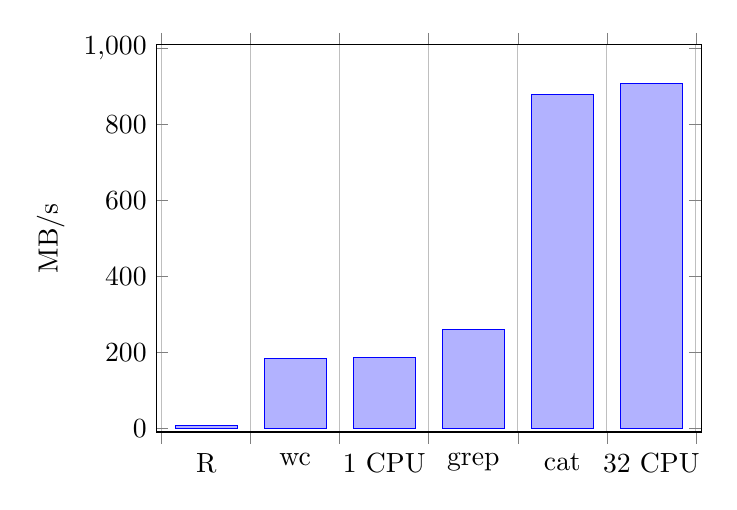
\begin{tikzpicture}
\begin{axis}[
	ylabel=MB/s,
  ymin=0, ymax=1000,
	enlargelimits=0.01,
	ybar interval=0.7,
  symbolic x coords={R, wc, 1 CPU, grep, cat, 32 CPU, end},
  width=8.5cm, height=6.5cm,
]
\addplot coordinates {(R,6.0) (wc,182.6) (1 CPU,186.6) (grep,261) (cat,878) (32 CPU,908) (end,0) };
% \addplot coordinates {(R,6.0) (wc,182.6) (CPU1,186.6) (grep,261) (wc -l,852) (cat,878) (Run 372,908) (Run 1,1029) (end,0) };

% \legend{MB/s}

\end{axis}
\end{tikzpicture}
\end{center}

\caption{Throughput comparisons of Icicle (1 CPU and 32 CPU) against existing R code and standard Unix utilities; higher is faster.}
\label{icicle:fig:bench:other}
\end{figure}



At Ambiata we are currently using Icicle in production over medium-sized data sets that fit on a single disk. We are also currently implementing a scheduler to distribute larger data sets across multiple nodes. The data we are working with is tens of terabytes compressed, which in 2016 does not fit on a single disk. However, each row has a natural primary key and the features we need to compute depend only on the data within single key groups, which makes the workload very easy to distribute.

% These initial results have been very promising, and we are currently implementing distribution across multiple machines to handle datasets that are tens of terabytes compressed, and do not fit on a single disk.
% Incremental computation is even more important for this distributed case, as we can avoid copying terabytes of data over the network.

In our proof of concept testing we replaced an existing R script that performed feature generation with new Icicle code. The R script computed features from a 317GB data set. It computed 12 queries over each of 31 input tables, for 372 query evaluations in total. The R script took 15 hours to run and consisted of 3,566 lines of code. The replacement Icicle version is only 191 lines of code and takes seven minutes to run.

The table in Figure~\ref{icicle:fig:bench:other} shows the throughput in megabytes per second.
We compared the throughput of several programs over the same dataset:
\begin{itemize}
\item our original R implementation (R);
\item Icicle running single-threaded (1 CPU);
\item Icicle running on multiple processors (32 CPU);
\item finding empty lines with @grep "^$"@;
\item counting characters, words and lines with @wc@;
\item reading and throwing away the results with @cat > /dev/null@.
\end{itemize}

We ran all the Unix utilities with unicode decoding disabled using @LANG=C LC_COLLATE@ for maximum performance. The input data does not contain unicode characters. 
We used an Amazon EC2 @c3.8xlarge@ with 32 CPUs, 60GB of RAM, and striped, RAIDed SSD storage. The fused Icicle version significantly outperformed the R version of the queries, and the single-threaded version was on par with @wc@, while only a little slower than @grep@. This is despite the fact that the Icicle queries perform more computational work than @wc@ and @grep@. By using multiple processors, we were able to scale up to perform as well as @cat@, approaching the disk speed.
The memory usage of Icicle starts at around 200MB of RAM for a single thread, but as more threads are added approaches 15MB per thread.
The memory usage is constant in the input size and depends on the number of queries.
The R code is single threaded and would require at least 150 processors to reach similar speeds, assuming perfect scaling.
These results give us confidence that our distributed implementation will be fast as well as scalable~\cite{mcsherry2015scalability}.


% The R code requires an @i2.8xlarge@ with 244GB of memory, but we were unable to perform our other benchmarks on such a large machine.
% \BEN{I wouldn't worry about stating this. You can't give out your R code so no one will test it themselves, and if even if you could run it on the smaller machine it wouldn't be faster}

% We were able to achieve such good results by generating parsing code specialised to the schema, and using data-only flattening~\cite{bergstrom2013data} as an efficient representation of structures such as arrays of sum types and tuples.
% \BEN{This isn't part of the contribution of this paper, so there's no real reason to discuss it}.

% By using a query plan that is close to a functional language, we are able to apply many standard optimisations such as common subexpression elimination and dead code removal.
% \BEN{We already said this before}. 



%!TEX root = ../Main.tex

\begin{figure}

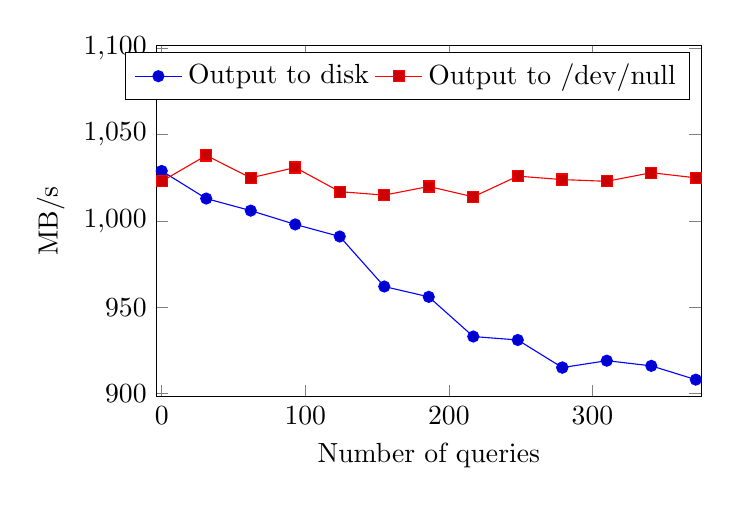
\begin{tikzpicture}
\begin{axis}[
	x tick label style={/pgf/number format/1000 sep=},
	ylabel=MB/s,
  ymin=900, ymax=1100,
%  xmax=372,
  xlabel=Number of queries,
	enlargelimits=0.01,
	legend style={legend columns=-1},
  width=8.5cm, height=6.05cm,
%	legend style={at={(0.5,-0.1)},anchor=north,legend columns=-1},
%	ybar interval=0.7,
]

% bench/raw.txt
% Running with fewer queries
% \addplot coordinates {(0,1025.5) (1,1029.6) (48,978) (96,941) (144,943) (192,936) (240,904) (276,895.5) (324,881) (372,846.2) };

% bench/raw.txt
% Running with fewer queries, better distribution
% \addplot coordinates { (0,1029) (31,1013) (62,1006) (93,998) (124,991) (155,941) (186,956) (217,933) (248,931) (279,915) (279,915) (310,919) (341,916) (372,908) };

%% APPLY LOPASS
\addplot coordinates { (0,1029) (31,1013) (62,1006) (93,998) (124,991) (155,962) (186,956) (217,933) (248,931) (279,915) (279,915) (310,919) (341,916) (372,908) };


% Fusion, no output
% \addplot coordinates { (0,1001) (31,1038) (62,1025) (93,1031) (124,1006) (155,1015) (186,1020) (217,997) (248,1026) (279,1024) (310,1009) (341,1038) (372,1025) };

%% APPLY LOPASS
\addplot coordinates { (0,1023) (31,1038) (62,1025) (93,1031) (124,1017) (155,1015) (186,1020) (217,1014) (248,1026) (279,1024) (310,1023) (341,1028) (372,1025) };

% No fusion, no output
% \addplot coordinates { (0,987) (31,1037) (62,1024) (93,1002) (124,1037) (155,1024) (186,1004) (217,1040) (248,1023) (279,998) (310,1018) (341,1013) (372,1003) };

\legend{Output to disk, Output to /dev/null};

\end{axis}
\end{tikzpicture}


\caption{Decrease in read throughput as queries are added, comparing writing the output to disk and writing to /dev/null.}
\label{icicle:fig:bench:queries}
\end{figure}


% \begin{figure}
% \begin{tikzpicture}
% \begin{axis}[
% 	x tick label style={/pgf/number format/1000 sep=},
% 	ylabel=MB/s,
%   ymin=0, ymax=1200,
%   xlabel=Number of threads,
% 	enlargelimits=0.01,
% 	legend style={legend columns=-1},
% ]
% \addplot coordinates { (1,163) (2,335) (3,442) (4,532) (5,578) (6,615) (7,633) (8,628) (9,631) (10,626) (11,637) (12,643) (13,658) (14,795) (15,781) (16,798) (17,840) (18,864) (19,862) (20,867) (21,847) (22,877) (23,876) (24,884) (25,862) };
% \end{axis}
% \end{tikzpicture}
% \caption{Scaling as threads are added}
% \label{icicle:fig:bench:scaling}
% \end{figure}




Figure~\ref{icicle:fig:bench:queries} shows how the total read througput scales as the number of fused queries is increased. For each number of queries, we ran two versions of the fused result: one version that wrote the output to disk, and the other that piped the result to @/dev/null@. The graph shows the throughput of the disk version decreasing roughly linearly in the number of queries, while the version ignoring the output remains constant. This suggests that we are IO bound on the write side. The time spent evaluating the queries themselves is small relative to our current IO load, and we are curently scaling up our system to use a larger query set.

% This suggests that the output code is the bottleneck, which is unsurprising given the output format is text-based PSV.
% computing the queries appears constant as hundreds of queries are added, which suggests that many more queries can be handled if a better output format is used.
% \BEN{I don't understand this, surely the program would produce the PSV even if it was just sent to /dev/null?}

%!TEX root = ../Main.tex
\section{Discussion}
\label{icicle:s:Conclusion}

% This paper has introduced Icicle, a streaming query language. The streaming, single-pass nature of Icicle allows all queries over the same table to be fused into a single loop over the data.
% Icicle's modal type system allows incremental computation, ensuring that queries give the same value regardless of how the input is sliced up, and when the increments are performed.
% The modal types encode when computations are available, and disallows using the results of folds before they are finished.
% \ben{the above paragraph doesn't add any new information}.

In Icicle, as in the push streams from \cref{taxonomy/push}, there is only one input stream, sourced from the input table, which is implicit in the bodies of queries.
This approach is intentionally simpler than existing synchronous data flow languages such as Lucy~\cite{mandel2010lucy} and fusion techniques using synchronous data flow such as flow fusion~\cite{lippmeier2013data}.
Synchronous data flow languages implement Kahn networks~\cite{vrba2009kahn} that are restricted to use bounded buffering~\cite{johnston2004advances} by clock typing and causal analysis~\cite{stephens1997survey}.
In such languages, stream combinators with multiple inputs, such as @zip@, are assigned types that require their stream arguments to have the same clock --- meaning that elements always arrive in lockstep and the combinators themselves do not need to perform their own buffering.
In Icicle the fact that the input stream is implicit and distributed to all combinators means that we can forgo clock analysis.
All queries in a program execute in lock-step on the same element at the same moment, which ensures that fusion is a simple matter of concatenating the components of the loop anatomy of each query.

Short-cut fusion techniques such as foldr/build~\cite{gill1993short} and stream fusion~\cite{coutts2007stream} rely on inlining to expose fusion opportunities.
In Haskell compilers such as GHC, the decision of when to inline is made by internal compiler heuristics, which makes it difficult for the programmer to predict when fusion will occur.
In this environment, array fusion is considered a ``bonus'' optimisation rather than integral part of the compilation method.
In contrast, for our feature generation application we really must ensure that multiple queries over the same table are fused, so we cannot rely on heuristics.

StreamIt~\cite{thies2002streamit} is an imperative streaming language which has been extended with dynamic scheduling~\cite{soule2013dynamic}.
Dynamic scheduling handles data flow graphs where the transfer rate between different stream operators is not known at compile time.
Dynamic scheduling is a trade-off: it is required for stream operators such as grouping and filtering where the output data rate is not known statically, but using dynamic techniques for graphs with static transfer rates tends to have a performance cost.
Icicle includes grouping and filtering operators where the output rates are statically unknown, however the associated language constructs require grouped and filtered data to be aggregated rather than passed as the input to another stream operator.
This allows Icicle to retain fully static scheduling, so the compiled queries consist of straight line code with no buffering.

Icicle is closely related to work in continuous and shared queries.
A continuous query is one that processes input data which may have new records added or removed from it at any time.
The result of the continuous query must be updated as soon as the input data changes.
Shared queries are ones in which the same sub expressions occur in several individual queries over the same data, and we wish to share the results of these sub expressions among all individuals that use them.
For example, in \citet{munagala2007optimization}, input records are filtered by a conjunction of predicates, and the predicates occur in multiple queries.
\citet{madden2002continuously} uses a predicate index to avoid recomputing them.
\citet{andrade2003efficient} describes a compiler for queries over geospacial imagery that shares the results of several pre-defined aggregation functions between queries.
Continuous Query Language (CQL)~\cite{arasu2002abstract,stream2003stream} again allows aggregates in its queries, but they must be builtin aggregate functions.
Icicle addresses a computationally similar problem, except that our input data sets can only have new records added rather than deleted, which allows us to support general aggregations rather than just filter predicates.
It is not obvious how arbitrary aggregate functions could be supported while also allowing deletion of records from the input data --- other than by recomputing the entire aggregation after each deletion.


% How to architect a query compiler~\cite{shaikhha2016architect}.
% Scheduling dynamic dataflow~\cite{buck1993scheduling}.
% Co-iterative characterization~\cite{caspi1998co}.



